%%%% PROCESAR con PdfLaTeX !!!!!


\documentclass[12pt]{book}
\usepackage[T1]{fontenc}
\usepackage{lmodern}
\usepackage{geometry}\geometry{top=2cm,bottom=2cm,left=1cm,right=1cm}
\usepackage{amssymb}
\usepackage{amsmath}
\usepackage{graphicx}
%\usepackage{txfonts}
%\usepackage{hyperref}
\usepackage[hidelinks]{hyperref}
\usepackage[spanish]{babel}
\setcounter{tocdepth}{4}
\usepackage[usenames]{color}
\usepackage{pdfpages}
\usepackage{enumerate}
\usepackage{framed}
\usepackage{color}
\usepackage{wrapfig}\definecolor{shadecolor}{RGB}{224,238,238}


\usepackage[hidelinks]{hyperref}
\hypersetup{
    colorlinks=true,
    linkcolor=blue,
    filecolor=magenta,      
    urlcolor=cyan,
    pdftitle={Sharelatex Example},
    bookmarks=true,
%    pdfpagemode=FullScreen,
}

\begin{document}
\thispagestyle{empty}

\begin {center}


\includegraphics[scale=.4]{Logo-fcenuba.png}

\medskip
\textbf{Facultad de Ciencias Exactas y Naturales}
\\
Universidad de Buenos Aires
\\
Departamento de Matemáticas

\vspace{3cm}


\textbf{\large Álgebra I}\\
\textbf{Segundo Cuatrimestre 2020}
\\    Guia Pr\'actica 5
\\ Ejercicios entregables
\vspace{2cm}




\end {center}


\vspace{2.5cm}

\noindent Isaac Edgar Camacho Ocampo
 

\vspace{1cm}

\vspace{1cm}

\noindent Buenos Aires, 2020

\newpage

\tableofcontents


\chapter{Práctica 1 - Conjuntos, Relaciones y Funciones}
\section{Guia 1}
%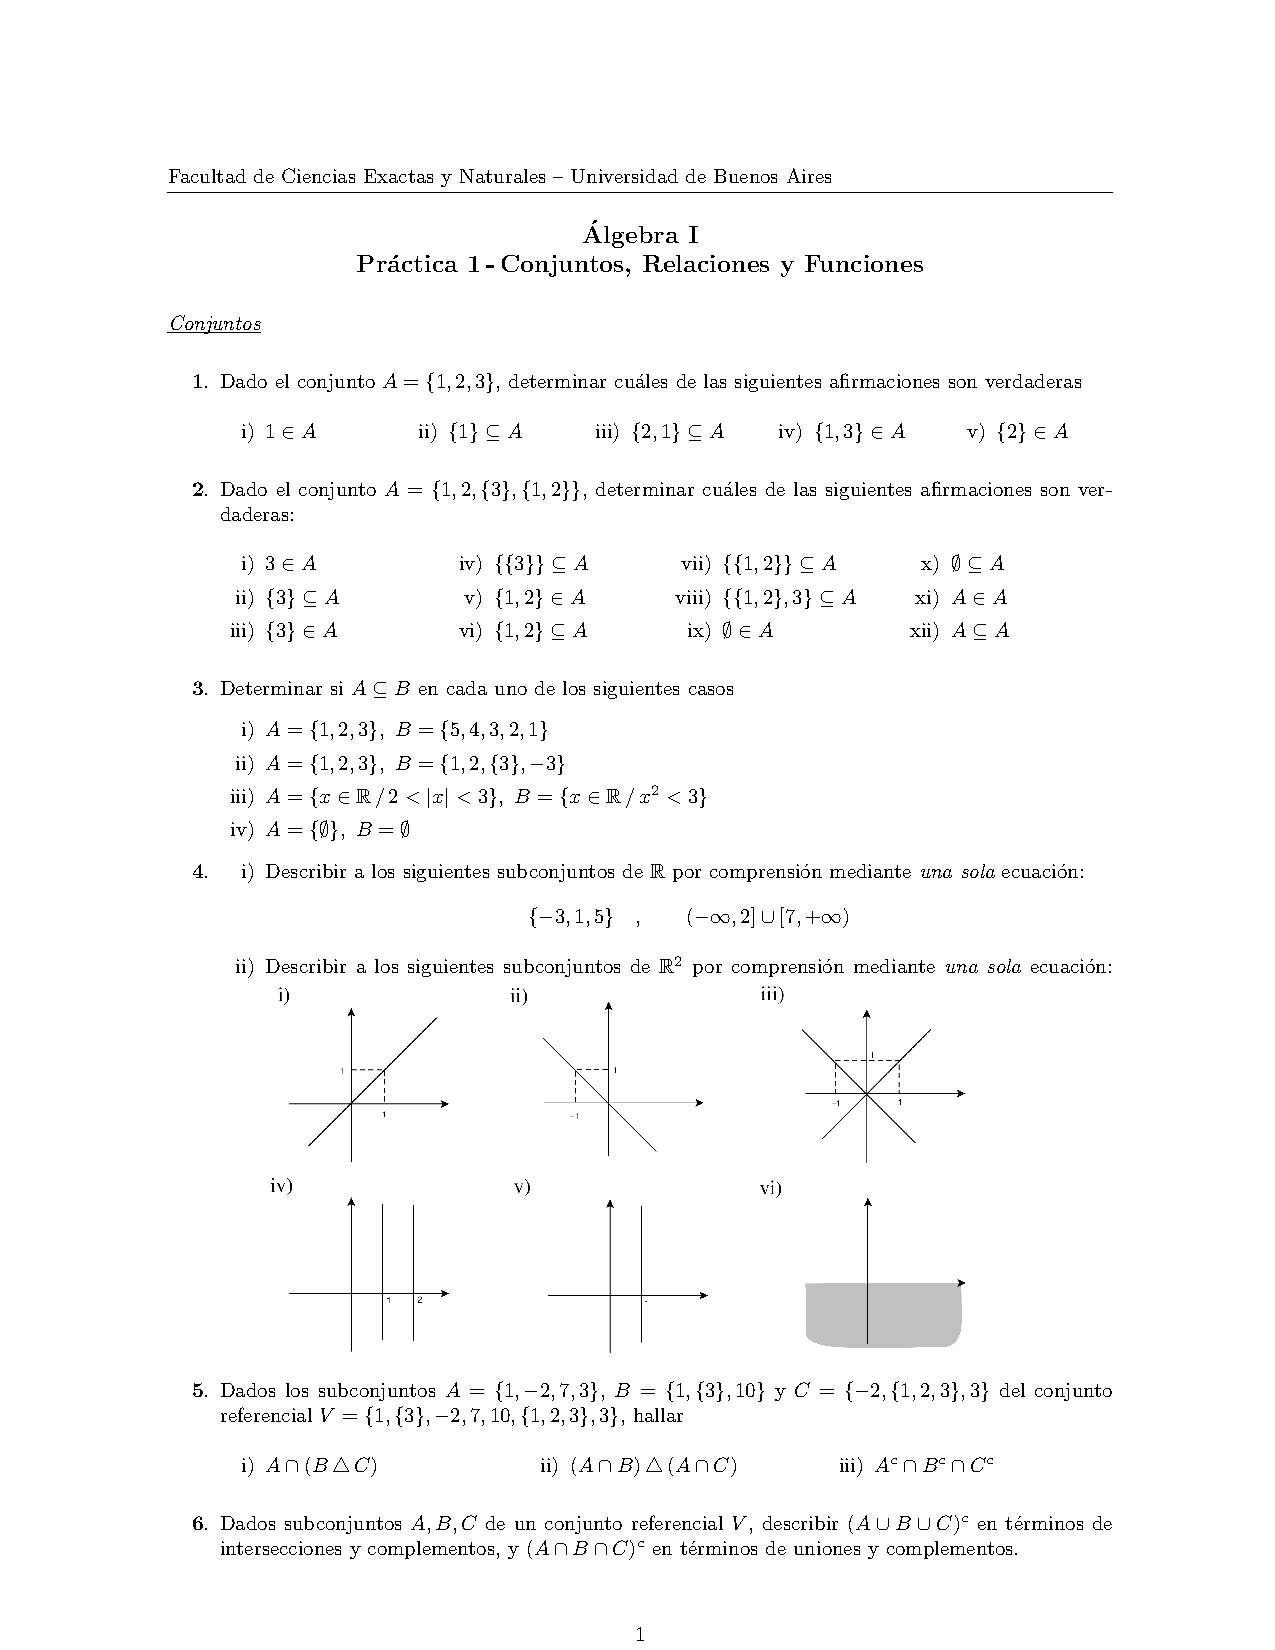
\includepdf[pages=-]{./pdfs/Practica1.pdf}


\section{Resoluci\'on}
\begin{enumerate}
\item 
	\begin{enumerate}[i]
	\item \textbf{verdadero} de forma trivial.
	\item \textbf{verdadero}, Recordar que $ \{ C \subseteq D \Leftrightarrow \forall x \in C \Rightarrow x \in D \} $ y podemos ver 			que 1 esta en ambos connjuntos.
	\item \textbf{verdadero}, el razonamiento es id\'entico, solo hay que tener en cuenta que para conjuntos no es 				relevante 	ni las repeticiones de elementos ni el \'orden.
	\item \textbf{falso}, porque el conjunto cuyos \'unicos elementos son 1,3 no esta en A, $ \{ 1, 3\} \notin A $ aqui 			hay que tener en cuenta que se esta usando el pertenece y no la inclusi\'on de conjuntos.
	\item \textbf{falso} por la misma raz\'on que el item anterior.
	\end{enumerate}
\item 2
\item 3
\item 4
\item 	
	\begin{enumerate}[i]
	\item \textbf{Recordemos que} $B \vartriangle C $ son todos los elementos que estan en B o en C pero no en ambos.\\
		$B\vartriangle C = \{ 1, \{ 3 \}, 10, -2, \{1, 2, 3\}, 3 \} $ \\
		$ A\cap (B\vartriangle C ) = \{ 1, -2, 3\}$ \\ 
		
	\item $ A\cap B = \{ 1\} $ y $ A\cap C = \{ -2,3\}  \Rightarrow  (A\cap B) \vartriangle (A\cap C ) =  \{1, 					-2,3\} $ \\
	Notar que el resultado es igual que I porque $ A\cap (B\vartriangle C ) =  (A\cap B) \vartriangle (A\cap C )$
	ambos resultados son equivalentes solo hay que distribuir.\\
	
	\item \textbf{Usando la ley de De Morgan} 
	\begin{align*}
	A^{c} \cap B^c \cap C^c = (A\cup B\cup C)^c & \Rightarrow A \cup B\cup C = \{1, \{3\}, -2, 7, 10, \{1, 2, 3\}, 3\} \\
	&\Rightarrow (A\cup B\cup C) =  V  \\
	&\Rightarrow (A\cup B\cup C)^c = \lbrace \emptyset \rbrace
	\end{align*}
	
	\end{enumerate}
	\item 6
	\item 7
	\item 
	\begin{enumerate}[i]
	\item Podemos ver a la parte subrayada del gr\'afico como la uni\'on de tres conjuntos, \\
	$ A \cup \{ (A\cap C) - B\} \cup \{(B\cup C) - A \}$
	\item Este es claramente la diferencia sim\'etrica entre A y C, quitandole ademas todos lo elementos de B \\
	$ (A \bigtriangleup C) - B $
	\item Tambien lo podemos mirar como la uni\'on de tres subconjuntos \\
	$ \{ (A \cap B)-C\} \cup \{ (B \cap C)-A\} \cup \{ (A \cap C)-B\}   $
	\end{enumerate}
	
	\item 9
	\item 
		\begin{align*}
			P(A) \subseteq P(B)	\qquad &\Rightarrow \qquad A \subseteq B \\
			A \underbrace{\subseteq}_{definicion} \textit{P}(A) \qquad  &\Rightarrow \qquad A	
				\underbrace{\subseteq}_{Hip\'otesis} \textit{P}(B) \\
			\text{ Pero } P(B) \subseteq B \text{ ya que } \qquad \forall x \in P(B) \qquad &\Rightarrow \qquad x \in B \\
			&\Rightarrow A \subseteq B \\ \\
			A \subseteq B \qquad &\Rightarrow \qquad P(A) \subseteq P(B)	\\
			\forall x \in A \qquad &\Rightarrow \qquad x \in P(A) \\
			\forall x \in A \qquad &\Rightarrow \qquad x \in B \subseteq P(B) \\
			\forall x \in P(A) \qquad &\Rightarrow \qquad x \in P(B) \\
			& 	\Rightarrow P(A) \subseteq P(B)
		\end{align*}
	\item 11	
	\item 

\begin{enumerate}[i]
	\item 
\begin{enumerate}[a)]
	\item \textbf{falso}, tomar el contraejemplo, n = 2.
	\item \textbf{verdadero}, porque me dice que existe alg\'un n natural que cumple la condici\'on, no es una proposici\'on categ\'orica, sino singular.
	\item \textbf{verdadera}, porque los intervalos incluyen a todos los Naturales, $[5, + \infty] \cup [1,8]$
	\item \textbf{verdadera}, porque no es un intervalo vac\'io $ [5,8] \neq \emptyset$
	\item \textbf{verdadera}, porque cualquiera sea n, eligiendo m = n+1 se verifica la proposici\'on.
	\item \textbf{falso}, lo que me quiere decir, es que existe un n que verifica, que es menor estr\'icto para todo m, y eso es falso porque si n = 1, y m = 1 $ \Rightarrow $ 1 no es menor estricto que 1.
\end{enumerate}	
	
	\item 
	\item 
	\end{enumerate}
	\item 13				
	\item 14
	\item 15
	\item 16
	\item 17 R = {(1, 1), (1, 3), (1, 7), (3, 1), (3, 5)}
	\item %ejercicio 18

\begin{enumerate}[i)]
	\item \textbf{verdadero}
	\item \textbf{falso}, porque en el elemento (3, 2),  $2 \notin B $
	\item \textbf{verdadera}
	\item \textbf{verdadera}
	\item \textbf{verdadera}
	\item \textbf{verdadera}
\end{enumerate}	

	\item %ejercicio 19

\begin{enumerate}[i)]
	\item 	$	R = \{ (1, 1), (1, 3), (1, 5), (1, 7),(2,2),(2, 3), (2, 5), (2, 7),(3,3),(3, 5), (3, 7) \} $
	\item $	R = \{ (2, 1), (3,1) \} $
	\item $	R = \{ (2, 1), (2,3), (2,5), (2,7) \} $
	\item $	R = \{ (1, 7), (2, 5),(2,7), (3, 5), (3, 7) \} $
\end{enumerate}	

	\item %ejercicio 20
	\item %ejercicio 21
	
	\item %ejercicio 30
\textbf{Ejercicio 18}
\begin{enumerate}[i)]
	\item \textbf{No es funci\'on} porque el 1 tiene varias imagenes.
	\item \textbf{no es funci\'on} idem.
	\item \textbf{no es funci\'on}
	\item \textbf{no es funci\'on}
	\item \textbf{si es funci\'on} $ \forall x \in A \Rightarrow \ \exists ! 	\ y \in B \ \ \vert (x,y) \in R$
	\item \textbf{si es funci\'on}
\end{enumerate}	
		
\end{enumerate}
	
\chapter{Práctica 2 - Números Naturales e Inducción} 
%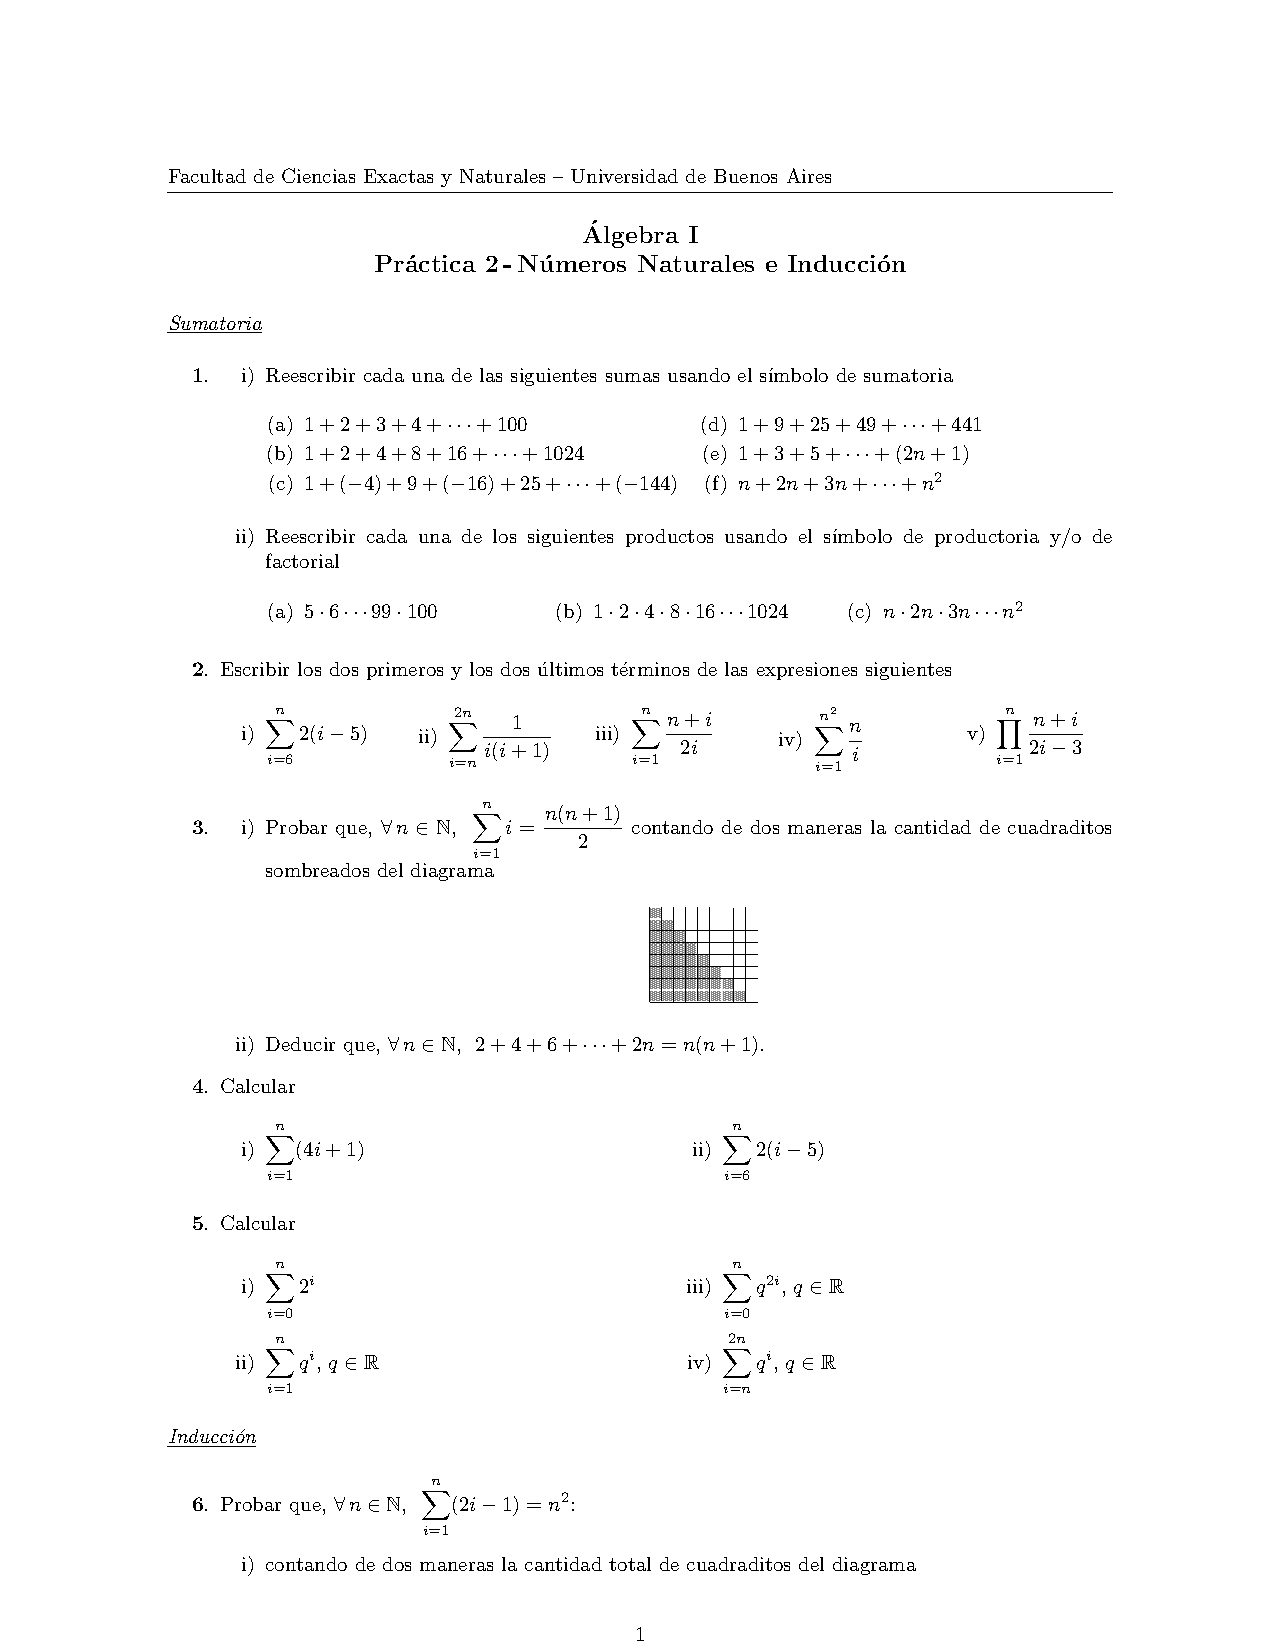
\includepdf[pages=-]{./pdfs/Practica2.pdf}


\section{Resoluci\'on}
\begin{enumerate}
\item 
	\begin{enumerate}[i)]
	\item % ejercicio 1	
	\begin{enumerate}[a)]
	\item $ \sum_{i=1}^{100}i $ \qquad (es la sumatoria trivial).
	\item $ \sum_{i=1}^{11}2^{i-1} $ 	
	\item $ \sum_{i=1}^{12}(-1)^{i-1} \cdot i^2 $		
	\item $ \sum_{i=1}^{21}(2i-1)^{2} $ 	
	\item $ \sum_{i=0}^{n}(2i+1) $ 		
	\item $ \sum_{i=1}^{n}(i\cdot n) $ 			
	\end{enumerate}
	
	
	
	\item % ejercicio 2
	
	\begin{enumerate}[a)]
	\item $ \prod_{i=5}^{100}i=5\cdot 6\cdots 100  $ 
	\item $ \prod_{i=0}^{10}2^i $ 
	\item $ \prod_{i=1}^{n}(i \cdot n) $ 	
	\end{enumerate}
	
	
	\end{enumerate}
\item %ejercicio 2
	\begin{enumerate}[i)]
	\item
\[
\sum_{i=6}^{n}2(i-5) = 2(6-5)+2(7-5)+ \cdots + 2(n-1-5)+2(n-5)
\]

	\item 

\[
\sum_{i=n}^{2n} \frac{1}{i(i+1)}= \frac{1}{n(n+1)} + \frac{1}{(n+1)(n+1+1)} + \cdots + \frac{1}{(2n-1)(2n-1+1)} + \frac{1}{2n(2n+1)}
\]
	
	\item 
\[
\sum_{i=1}^{n}\frac{n+i}{2i} = \frac{n+1}{2 \cdot 1}+\frac{n+2}{2 \cdot 2}+ \cdots + \frac{(n-1)+1}{2 \cdot (n-1)}+\frac{n+n}{2 \cdot n}
\]
	
	\item 
\[
\sum_{i=1}^{n^2}\frac{n}{i} = \frac{n}{1}+\frac{n}{2}+ \cdots + \frac{n}{(n-1)^2}+\frac{n}{n^2}
\]


	\item 
\[
\prod_{i=1}^{n}\frac{n+i}{2i-3} = \frac{n+1}{2\cdot 1-3} \cdot \frac{n+2}{2\cdot2 - 3} \cdots  \frac{n+(n-1)}{2(n-1)-3}\cdot \frac{n+n}{2n-3}
\]
		
	\end{enumerate}

\item %ejercicio 3

	\begin{enumerate}[i)]
	\item Usamos inducci\'on, primero para n=1
	\[ \sum_{i=1}^{1} i = 1 \text{ (ahora verificamos la f\'ormula ) } \frac{n(n+1)}{2} \text{, con n = 1, } \] 
	\[ \frac{1(1+1)}{2} = 1 \text{, se verifica la propiedad para n = 1. }	\Rightarrow P(1) = True\]
\\
\textbf{Hip\'otesis inductiva} \[ \sum_{i=1}^{n} i = \frac{n(n+1)}{2}\]
\\
\textbf{T\'esis inductiva} 
\begin{align*}
\sum_{i=1}^{n+1}i &= \frac{(n+1)(n+1+1)}{2} \\
\sum_{i=1}^{n+1}i &= \sum_{i=1}^{n}i + (n+1)\\
\underbrace{\sum_{i=1}^{n}i}_{\frac{n(n+1)}{2}} + (n+1) & \underbrace{=}_{ \text{por HI }} \frac{n(n+1)}{2} + (n+1) \\ \\
\frac{n(n+1)}{2} + (n+1) &= \frac{n(n+1) + 2(n+1)}{2} \qquad \text{ (factor com\'un (n+1))} \\
\frac{n(n+1) + 2(n+1)}{2} &= \frac{(n+1)(n+2)}{2} 
\end{align*}
\begin{shaded}
\[ \textbf{probamos que }\Rightarrow \sum_{i=1}^{n+1}i = \frac{(n+1)(n+1+1)}{2} \qquad \forall n \in \mathbb{N} \]
\end{shaded}
	\item De igual manera probaremos, por inducci\'on la igualdad \[ 2+4+6+\cdots+2n = \sum_{i=1}^{n} 2i = n(n+1)\] para ello probamos que cumple para n=1, $ P(1) \Rightarrow \sum_{i=1}^{1} 2i = 1(1+1) = 2$, luego probamos el paso inductivo, suponiendo que P(n) es verdadero, $\sum_{i=1}^{n} 2i = n(n+1)$ probamos que es verdadero P(n+1) o $ \sum_{i=1}^{n+1} 2i = (n+1)(n+2) $.\\
Partimos de $\sum_{i=1}^{n+1} 2i$ y trataremos de llegar l\'ogicamente a $ (n+1)(n+2) $,\\
 $ \Rightarrow \sum_{i=1}^{n+1} 2i = \sum_{i=1}^{n} 2i + 2(n+1) \text{ pero usando la HI, } n(n+1)+2(n+1)$ y sacando factor com\'un (n+1) llegamos a, $ (n+1)(n+2)$ 	que era justo lo que queriamos probar.
	\end{enumerate}

\item %ejercicio 4
\item %ejercicio 5
Se trata de una serie geom\'etrica.
\[ \sum_{i=0}^{n} 2^i = 1+2+4+6+\cdots+2^n\] si multiplico ambos miembros por 2 y resto convenientemente
\begin{align*}
 \sum_{i=0}^{n} 2^i &= 1+2+4+6+\cdots+2^n  \\
  2 \cdot (\sum_{i=0}^{n} 2^i) &= 2\cdot(1+2+4+6+\cdots+2^n) \\
  \rule{20mm}{0.2mm} &  \rule{60mm}{0.2mm} \\
 2 \cdot (\sum_{i=0}^{n} 2^i)-  (\sum_{i=0}^{n} 2^i)  &= (2+4+6+ \cdots +2^n+2^{n+1}) - (1+2+4+6+ \cdots +2^n) \\
 \sum_{i=0}^{n} 2^i &= 2^{n+1} -1
\end{align*}
\end{enumerate}


\chapter{Práctica 3 - Números enteros (Parte 2)}
\section{Guia 3}
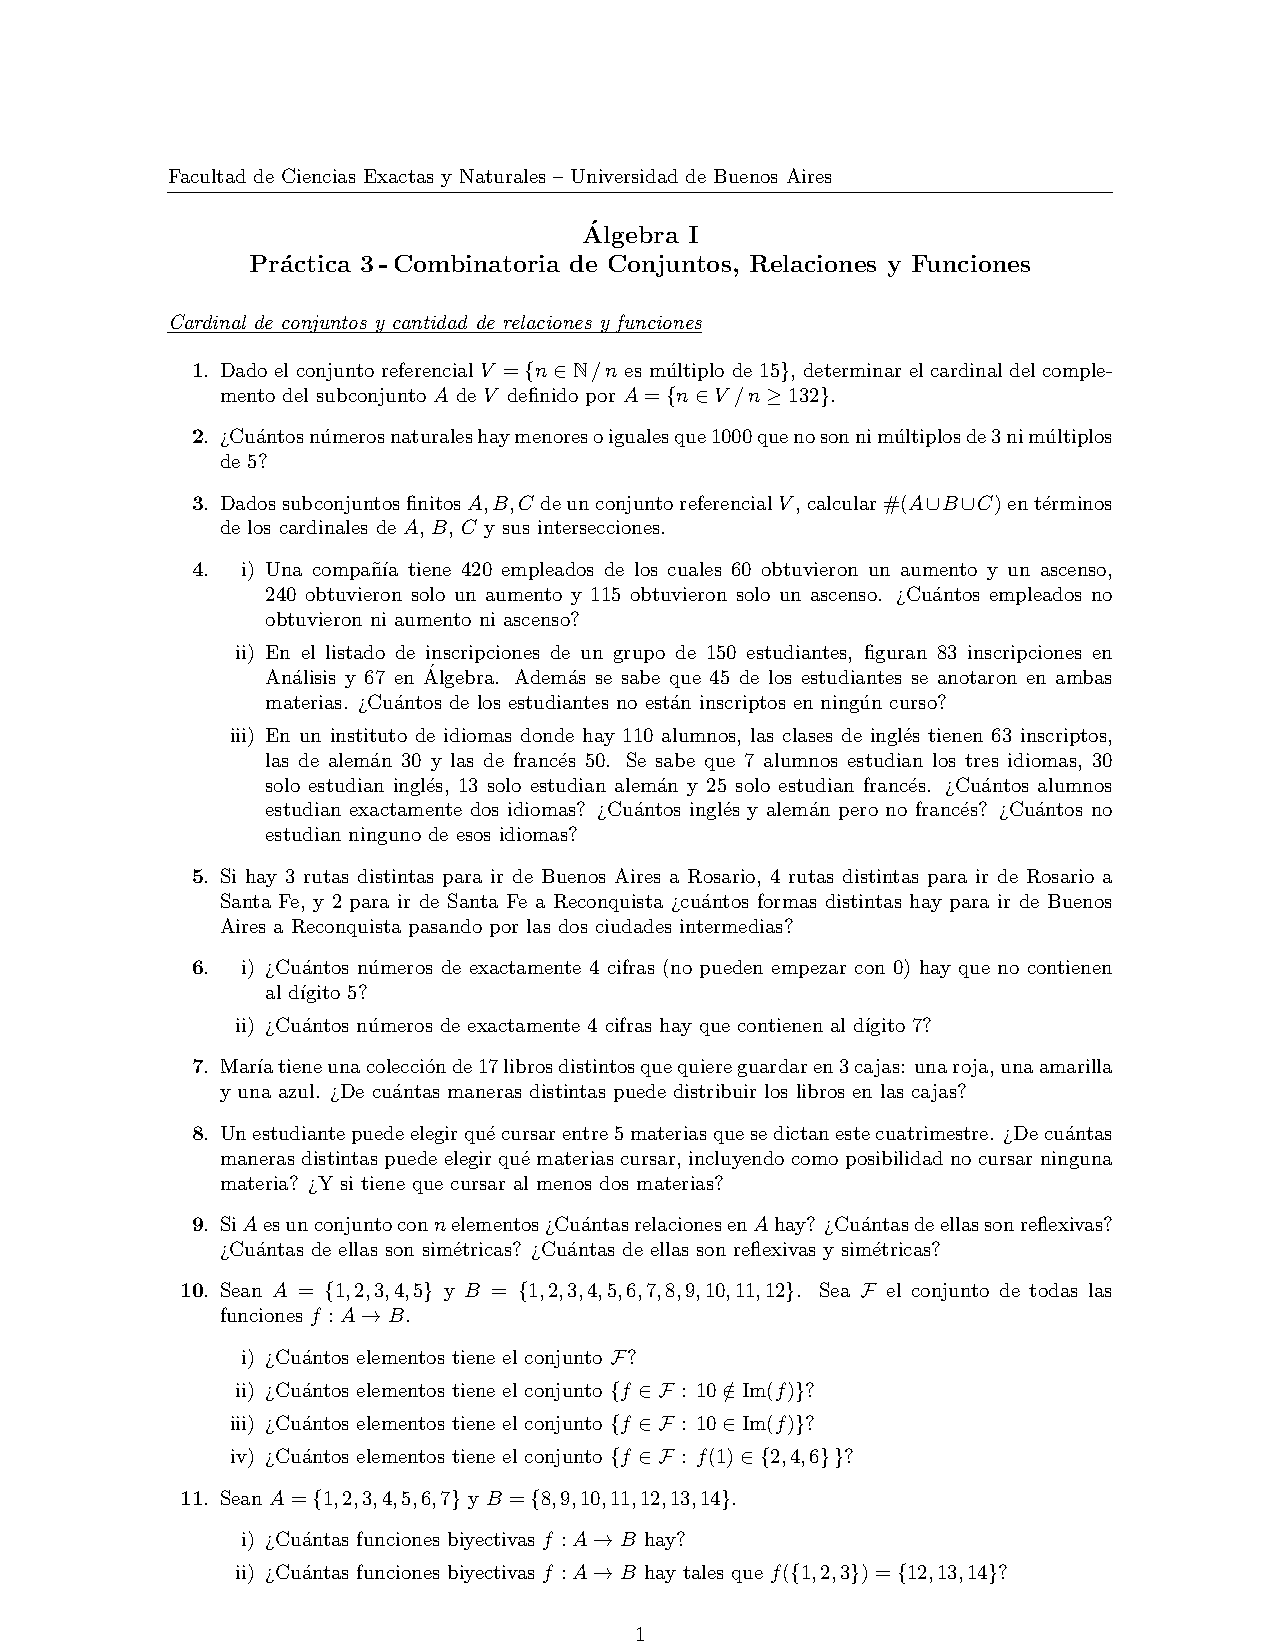
\includepdf[pages=-]{./pdfs/Practica3.pdf}


\section{Resoluci\'on}



\chapter{Práctica 4 - Números enteros (Parte 2)}
\section{Guia 4}
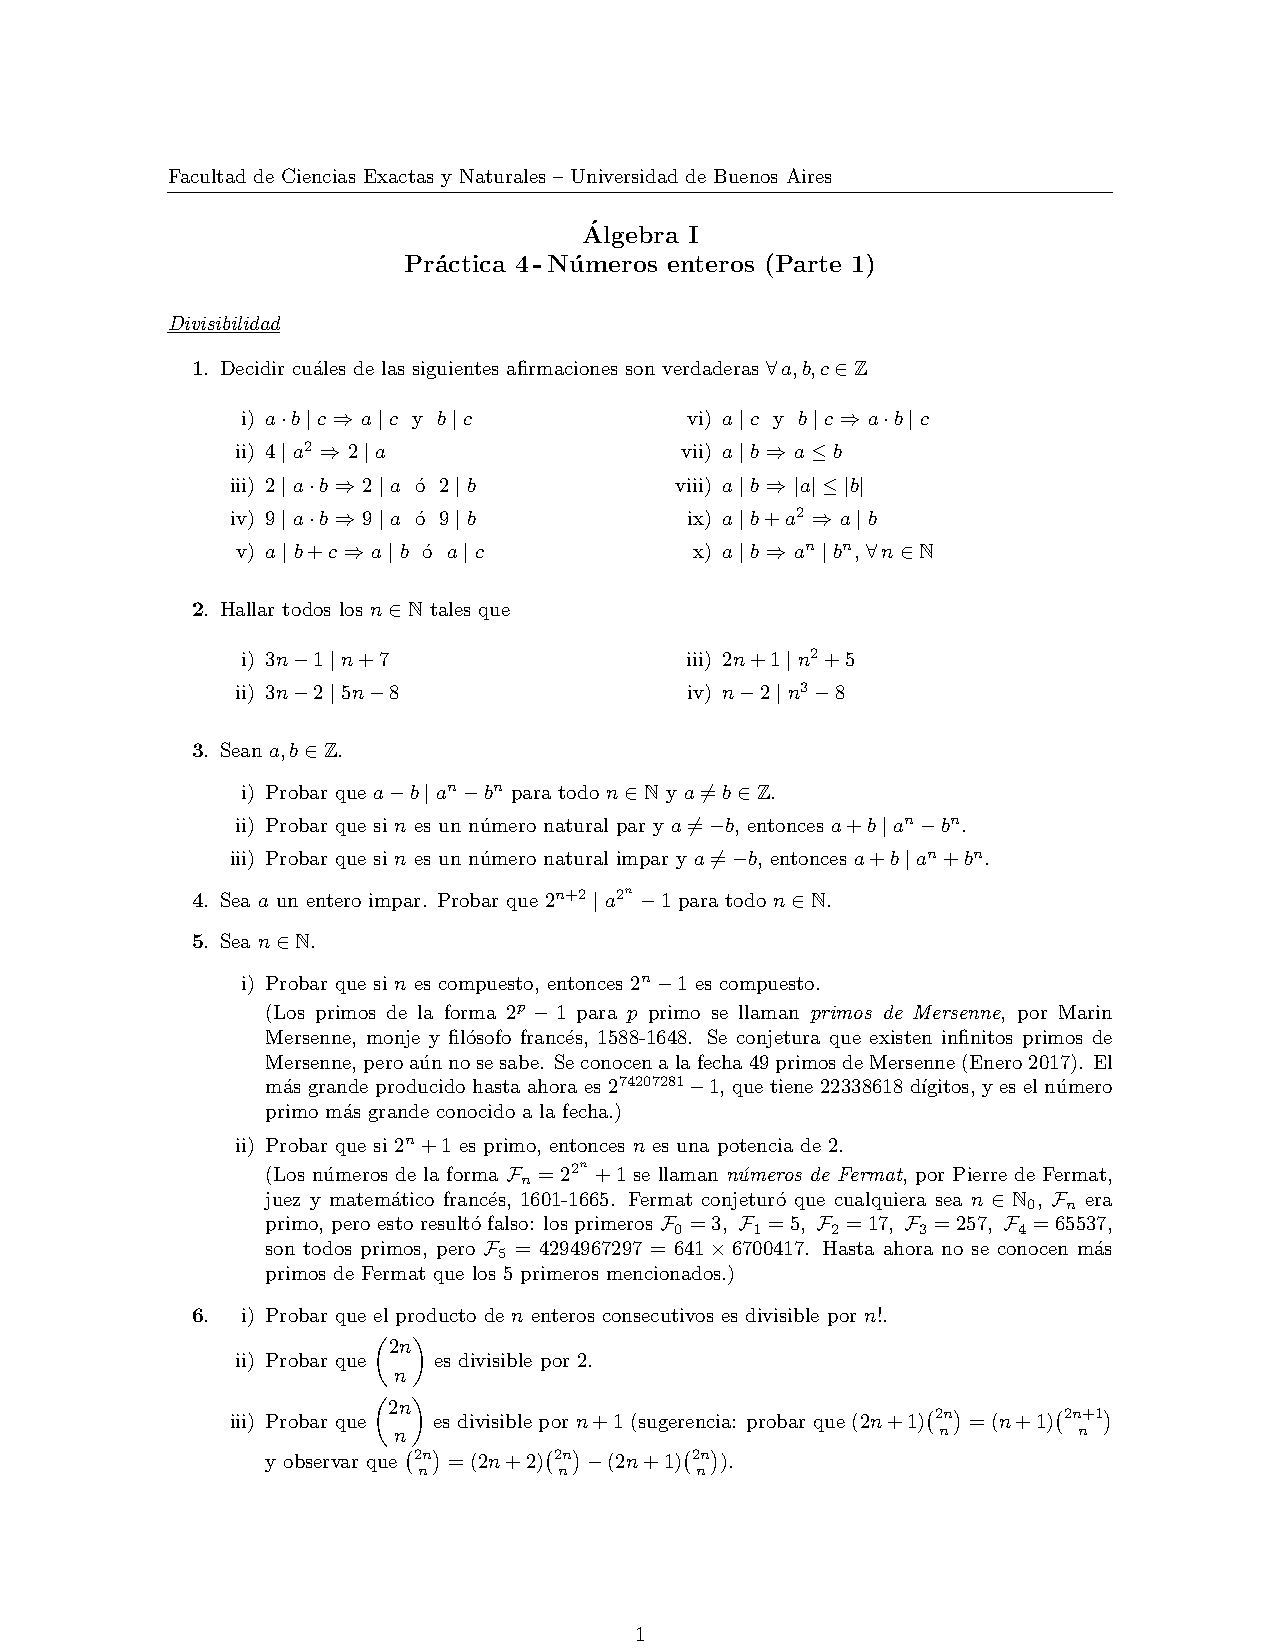
\includepdf[pages=-]{./pdfs/Practica4.pdf}


\section{Resoluci\'on}


\chapter{Práctica 5 - Números enteros (Parte 2)}
\section{Guia 5}
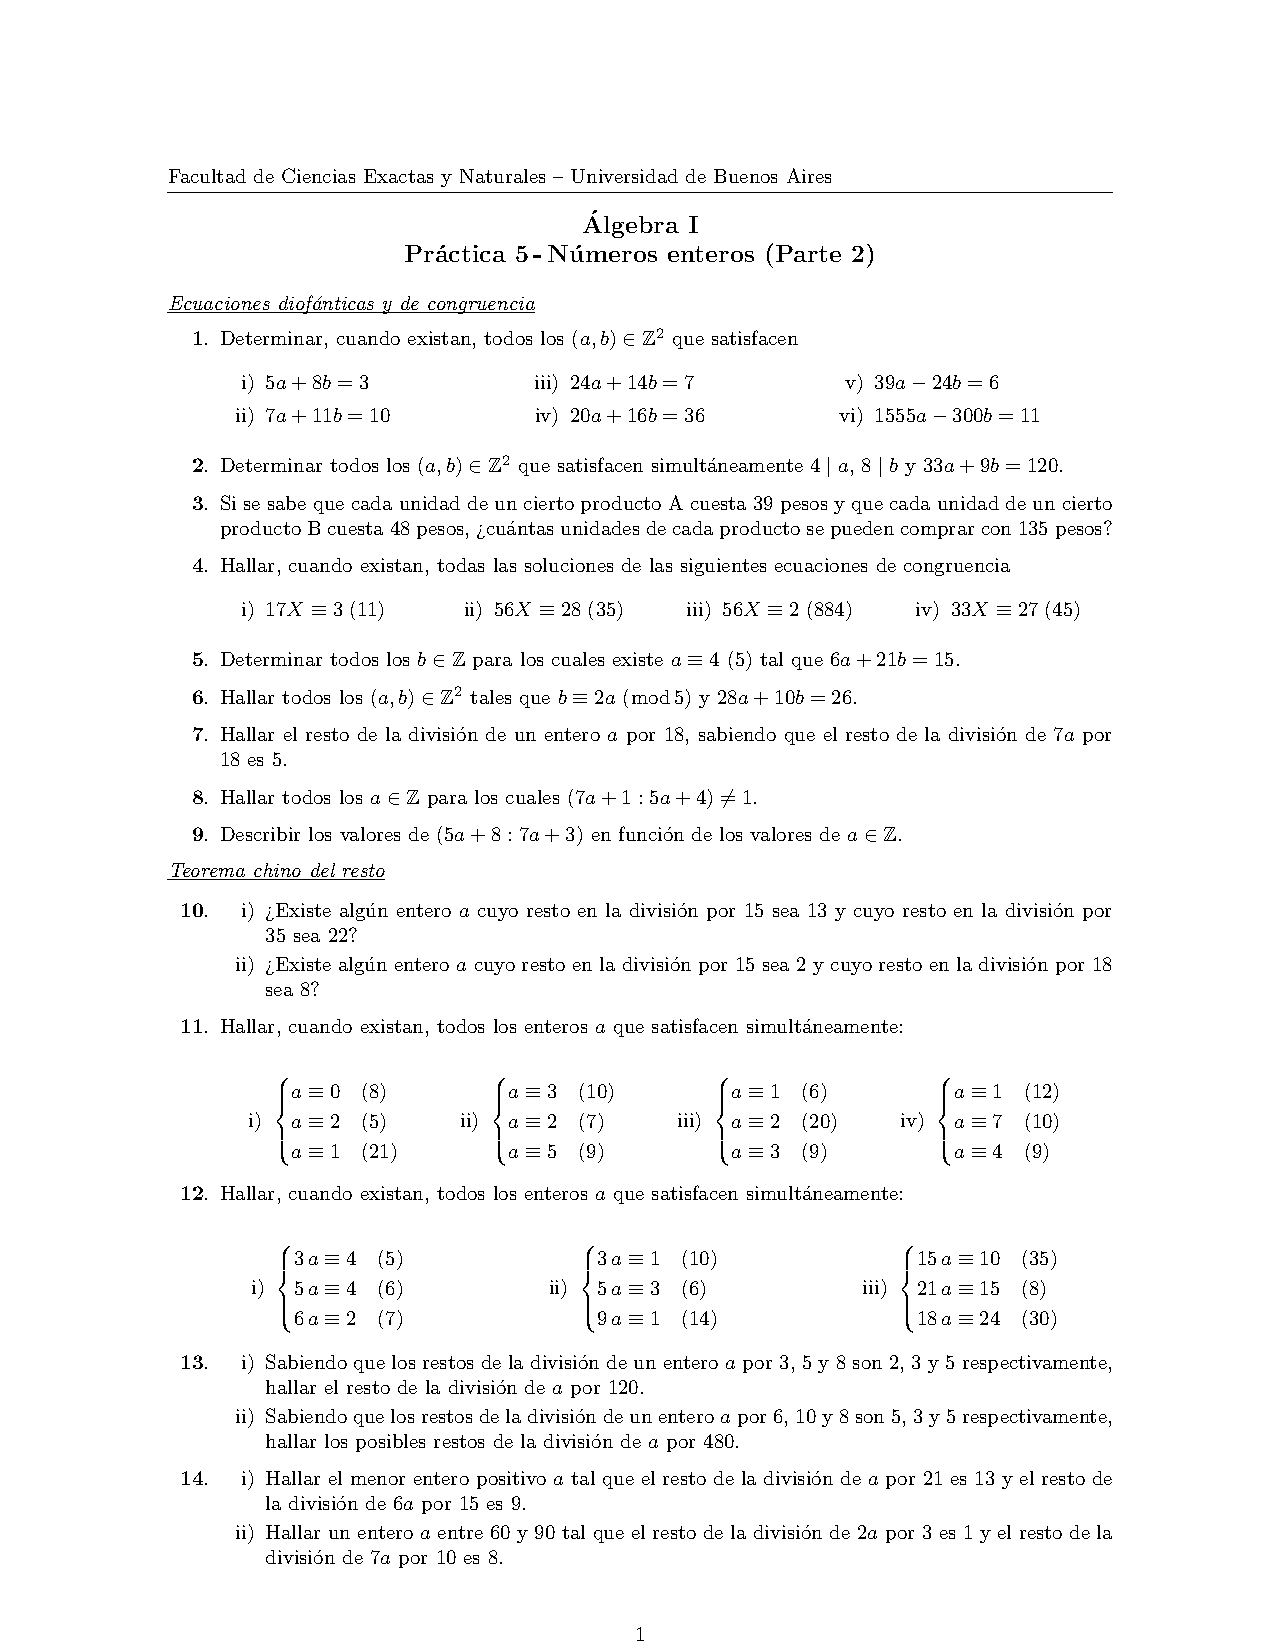
\includepdf[pages=-]{./pdfs/Practica5.pdf}


\section{Resoluci\'on}


hola mundo














\begin{shaded}
Para demostrar la corrección del programa en SmallLang con respecto a la especificación, debemos probar que:
\begin{align}
Post &\Rightarrow wp( \textbf{ c\'odigo previo al ciclo } , Pc) \\
Pc &\Rightarrow wp (\textbf{ ciclo}, Qc ) \\
Qc & \Rightarrow wp ( \textbf{ c\'odigo posterior al ciclo }, Post) 
\end{align}
La parte 2.2 con el teor\'ema del invariante. Si probamos estas tres implicaciones, por el principio de monoton\'ia sabemos que  $ Pre \Rightarrow wp(  programa completo  , Post)  $  y por lo tanto el programa  es correcto, respecto a su especificaci\'on
\end{shaded}

\section{Definici\'on de $ Qc, Pc, I, fv$}
Primero vamos a definir los predicados que necesitamos para la demostracion.
\begin{align*}
Pre & \quad \quad \{ True \}  \\
Post &= \quad \{ r = True \leftrightarrow ((\exists k :\mathbb{Z})(0 \leq k < |s|) \wedge_L s[k] = e)\} \\
Pc &= \quad (i = 0) \wedge (j = -1) \\
Qc &=  \quad(j \neq -1) \leftrightarrow (\exists k : \mathbb{Z})(0 \leq k < \mid s\mid \ \wedge_{L} \ s[k] = e) \\
I &= \quad 0 \leq i \leq  \mid s \mid) \wedge (j \neq -1) \leftrightarrow (\exists k : \mathbb{Z})(0 \leq k < i \rightarrow_L s[k] = e) \wedge (s[i] = e \rightarrow i = j)  \\
fv &= \quad ( \mid s \mid - i )\\
B &= \quad (i < \mid s \mid)
\end{align*}

\subsection{ Pre $\Rightarrow $ wp(código previo al ciclo, Pc )}
\begin{align*}
Pre \rightarrow wp(i:= 0; j := -1, Pc ) & \equiv \quad wp(i := 0; wp(j := -1, Pc )) \\ \\
Calculamos \ wp(j := -1, Pc ) & \\ 
wp(j := -1, Pc ) &\equiv \quad  def (-1) \wedge_L Pc_{-1}^j \\
 &\equiv \quad wp(j := -1, \left( (i = 0) \wedge (j = -1)\right)_{(-1)}^j ) \\
&\equiv \quad def (-1) \wedge (i = 0) \wedge (-1 = -1) \\
E1 &\equiv \quad  (i = 0) \\ \\
Calculamos \ wp(i := 0, E1) & \\
wp(i := 0, E1 ) &\equiv \quad  def (0) \wedge_L E1_{0}^i  \\
&\equiv \quad  True \wedge_L (i = 0)_{0}^i \\
&\equiv \quad (0 = 0) \\
E2 &\equiv \quad True 
\end{align*}
\begin{shaded}
Por lo tanto demostramos que: 
\begin{center}
$ Pre \Rightarrow wp( \textbf{ c\'odigo previo al ciclo } , Pc) $
\end{center}
\end{shaded}
\subsection{ Qc $\Rightarrow$ wp(if..then..else..fi, Post)}
\textbf{Recordamos la post } 
\[ Post = \{ r = True \leftrightarrow ((\exists k :\mathbb{Z})(0 \leq k < |s|) \wedge_L s[k] = e)\}  \]

Calculamos:
\begin{align*}
 wp(if ..... endif , Post) &\equiv wp(if ( j \neq -1) then \ r := True \ else \ r := False \ endif , Post)  \\
&\equiv def(j\neq -1) \wedge_L  \left[ (j \neq -1) \wedge wp(r := True , Post) \right] \vee \left[ (j = -1) \wedge wp(r := False, Post)\right]  \\
&\equiv \underbrace{def(j\neq -1)}_{\text{True}} \wedge_L \quad [ \qquad \qquad \qquad " \qquad \qquad \qquad ] \vee [\qquad \qquad \qquad " \qquad \qquad \qquad \qquad ]  \\
&\equiv (j \leq -1 \wedge wp(r := True, Post)) \vee (j = -1 \wedge wp(r := False, Post)) \\
&\equiv (j \leq -1 \wedge \textcolor{red}{wp(r := True, Post)}) \vee (j = -1 \wedge \textcolor{blue}{ wp(r := False, Post)}) 
\end{align*}
\begin{align*}
\textcolor{red}{wp(r := True, Post)} &\equiv def (True) \wedge_L Post_{true}^r \\
&\equiv (True = True) \leftrightarrow (\exists k : \mathbb{Z})(0 \leq k < |s| \wedge_L s[k] = e) \\
\textcolor{red}{wp(r := True, Post)} &\equiv (\exists k : \mathbb{Z})(0 \leq k < |s| \wedge_L s[k] = e) \\ \\  \\
\textcolor{blue}{ wp(r := False, Post)} &\equiv def (False) \wedge_L Post_{false}^r \\
&\equiv \underbrace{(false = True)}_{\text{False}} \leftrightarrow \underbrace{(\exists k : \mathbb{Z})(0 \leq k < |s| \wedge_L s[k] = e)}_{\text{(*)}} \\
(*) \ entonces \ como \ & (\exists k : \mathbb{Z})(0 \leq k < |s| \wedge_L s[k] = e)  \text{ debe ser Falso,  invierto desigualdad} \\ \\
\textcolor{blue}{ wp(r := False, Post)} &\equiv (\forall k : \mathbb{Z})(0 \leq k < |s| \wedge_L s[k] \neq e)\\ \\ \\ \\
wp(if... endif , Post) &\equiv (j \neq -1) \wedge ( \exists k : \mathbb{Z})(0 \leq k < |s| \wedge_L
s[k] = e) \vee \\ 
& \quad \ (j = -1) \wedge (\forall k :\mathbb{Z})(0 \leq k < |s| \wedge_L s[k] \neq e) \\
& \quad \ \textcolor{blue}{(aplico \ (p \wedge q) \vee (\neg p \wedge \neg q) \equiv p \leftrightarrow q)} \\
E3 &\equiv (j \neq -1) \leftrightarrow (\exists k :\mathbb{Z})(0 \leq k < |s| \wedge_L s[k] = e) 
\end{align*}
Chequeamos $Qc \rightarrow E3 $ 
\begin{align*}
Qc \equiv j \neq -1 & \leftrightarrow (\exists k : \mathbb{Z})(0 \leq k < |s| \wedge_L s[k] = e) \equiv E3
\end{align*}
\begin{shaded}
Por lo tanto demostramos que: 
\begin{center}
$Qc \Rightarrow E3$ 
\end{center}
\end{shaded}
\chapter{Demostraci\'on de la correcci\'on del ciclo}
\subsection{Qc $\Rightarrow$ wp(ciclo, Qc)}
\begin{shaded}
\textbf{Teorema}. Sean un predicado I y una funci\'on $ fv : \mathbb{V} \rightarrow \mathbb{Z} $
(donde $ \mathbb{V} $ es el producto cartesiano de los dominios de las variables del programa), y supongamos que I $ \rightarrow $ def(B). Si se cumplen: \\
\begin{align*}
\textbf{1)}\quad & PC \Rightarrow I, \\
\textbf{2)}\quad & \{I \wedge B \} S \{I \}, \\
\textbf{3)}\quad & I \wedge \neg B \Rightarrow Qc , \\
\textbf{4)}\quad & \{I \wedge B \wedge v_0 = fv \} S \{fv < v_0 \}, \\
\textbf{5)}\quad & I \wedge fv \leq 0 \Rightarrow \neg B, 
\end{align*}
... entonces la siguiente tripla de Hoare es v\'alida: \{PC \} while B do S endwhile \{QC \}
\end{shaded}
\subsection{$ Pc \ \rightarrow I $}
\begin{align*}
Pc &= \quad (i = 0) \wedge (j = -1) \\
I &= \quad 0 \leq i \leq  \mid s \mid) \wedge (j \neq -1) \leftrightarrow (\exists k : \mathbb{Z})(0 \leq k < i \rightarrow_L s[k] = e) \wedge (s[i] = e \rightarrow i = j) \\
&\equiv \quad (i = 0) \wedge (j = -1) \rightarrow ( 0 \leq i \leq  \mid s \mid) \  \checkmark (\textcolor{red}{trivial }) \\
&\equiv \quad (j\neq -1 \land (\exists k: \mathbb{Z})  ( 0\leq k <i \land_L s[k] = e ))  \lor  (j= -1 \land (\forall k: \mathbb{Z})  ( 0\leq k < i \land_L s[k] \neq e )) \checkmark 	
\end{align*}
( \textcolor{red}{porque  se cumple trivialmente que $ (j = -1) $ y por vacuidad $(j= -1 \land (\forall k: \mathbb{Z})  ( 0\leq k < i \land_L s[k] \neq e ))$ ya que no hay ningún número que sea mayor o igual a cero y menor a cero a la vez  }) 
\vspace{0.3cm}
\subsection{ $ (I \ \land \neg B) \rightarrow Qc$ }

\begin{align*}
Q_c &\equiv (j \neq -1)  \Leftrightarrow (\exists k: \mathbb{Z})(0 \leq k < |s| \land_L s[k] = e)  \\
B   &\equiv (i < |s|) \\
I &\equiv 0 \leq i \leq |s| \land j\neq -1 \Leftrightarrow (\exists k:\mathbb{Z})(0\leq k < i \Rightarrow_L s[k] = e)\wedge (s[i] = e \rightarrow i = j) \\ \\
& Q_c \checkmark 
\end{align*}
( \textcolor{red}{porque $I\land \neg B$ implica que $i = |s|$ ya que por $I $,  $ i \leq |s|$ y por $\neg B$\, $i \geq |s| $ y si aplico esto a $I$ me queda $Q_c$ }) 
\vspace{0.2cm}
\subsection{ \{$I\land B$\} ciclo  \{$I$\} }
\begin{align*}
I &= \quad (0 \leq i \leq  \mid s \mid) \wedge (j \neq -1) \leftrightarrow (\exists k : \mathbb{Z})(0 \leq k < i \rightarrow_L s[k] = e) \wedge (s[i] = e \rightarrow i = j) \\
B &\equiv \quad  (i < |s|) \\
\end{align*}
\begin{shaded}
\begin{align*}
& \textbf{Ciclo} \\
& \qquad if (s[i] = e)  then  \\
& \qquad \qquad j:= i \\
& \qquad else \\
& \qquad \qquad skip \\
& \qquad endif \\
& \qquad i:= i + 1 
\end{align*}
\end{shaded}
Veamos si $ (I \land B) \Rightarrow wp( $if...then..else..fi,  $ i := i +1, I ) $

\begin{align*}
wp( if..fi,   i := i +1, I )  \ &\equiv \ wp( if..fi,  \underbrace{ wp( i := i +1, I)}_{debo \ calcular} ) \\ \\
wp( i := i +1, I) \ &\equiv \  \underbrace{def(i+1)}_{True} \land_L I_{i+1}^i \\
&\equiv  (0\leq i +1 \leq|s|) \land_L ( j\neq -1 \Leftrightarrow (\exists k: \mathbb{Z})) ( 0 \leq k < i + 1 \Rightarrow_L s[k] = e)) \wedge \\
& \quad \ (s[i+1] = e \rightarrow i+1 = j)  \\ \\
E4 &\equiv  (0\leq i +1 \leq|s|) \land_L ( j\neq -1 \Leftrightarrow (\exists k: \mathbb{Z})) ( 0 \leq k < i + 1 \Rightarrow_L s[k] = e))\wedge \\
& \quad \  (s[i+1] = e \rightarrow i+1 = j)  \\
\end{align*}
\textbf{Calculo} $wp( if...then..else..fi,  E4 )$ \\
\begin{align*}
wp( if..fi,  E4 ) &\equiv \underbrace{ def(s[i] = e )}_{True} \land_L 
 \ \left[ \ s[i] = e \land wp(j := i, E4)  \ \right] \lor \left[ \ s[i] \neq e \land wp(skip, E_4)\right] \\
&\equiv (s[i] = e \land \underbrace{ def(i)}_{True} \land {E4}^j_i) \lor (s[i] \neq e \land E4) \\
&\equiv (s[i] = e \land  {E4}^j_i) \lor (s[i] \neq e \land E4) \\
&\equiv  (s[i] = e ) \quad \land  \\ 
& \quad \ (0\leq i +1 \leq|s|) \land_L ( i \neq -1 \Leftrightarrow (\exists k: \mathbb{Z})) ( 0 \leq k < i + 1 \Rightarrow_L s[k] = e))\wedge \\
& \quad \  (s[i+1] = e \rightarrow i+1 = i) \qquad \lor \\ 
& \quad \ (s[i] \neq e) \quad  \land \\
& \quad \ (0\leq i +1 \leq|s| \land_L ( j\neq -1 \Leftrightarrow (\exists k: \mathbb{Z}) ( 0 \leq k \leq i + 1 \Rightarrow_L s[k] = e))\wedge \\
& \quad \  (s[i+1] = e \rightarrow i+1 = j) \\ \\ \\
E5 &\equiv ( 0\leq i +1 \leq|s|) \land_L  \\
& \quad \ (s[i] = e \land (i\neq -1 \Leftrightarrow (\exists k: \mathbb{Z}) ( 0 \leq k < i + 1 \Rightarrow_L s[k] = e)) \wedge \\
& \quad \  (s[i+1] = e \rightarrow i+1 = i))\\
& \quad \ \lor \\  
& \quad \ (s[i] \neq e \land ( j\neq -1 \Leftrightarrow (\exists k: \mathbb{Z}) ( 0 \leq k \leq i + 1 \Rightarrow_L s[k] = e)) \wedge \\
& \quad \  (s[i+1] = e \rightarrow i+1 = j) ) \\ \\
\text{ Segun el invariante } & (s[i] = e \rightarrow i = j), \text{y usando la equivalencia }(p \wedge q )\vee(\neg p \wedge q )\equiv q \\ \\
E5 &\equiv ( 0\leq i +1 \leq|s|) \land_L  \\
& \quad \ ( \underbrace{ s[i] = e }_{\text{por I}}\land (\underbrace{ i \neq -1}_{\text{i=j}} \Leftrightarrow (\exists k: \mathbb{Z}) ( 0 \leq k < i + 1 \Rightarrow_L s[k] = e)) \wedge \\
& \quad \  (s[i+1] = e \rightarrow \underbrace{ i+1 = i }_{i=j}) )\\
& \quad \   \lor \\  
& \quad \ (s[i] \neq e \land ( j\neq -1 \Leftrightarrow (\exists k: \mathbb{Z}) ( 0 \leq k \leq i + 1 \Rightarrow_L s[k] = e)) \wedge \\
& \quad \  (s[i+1] = e \rightarrow i+1 = j) )\\ \\
E5 &\equiv ( 0\leq i +1 \leq|s|) \land_L  \\
& \quad \ ( s[i] = e \land ( j \neq -1 \Leftrightarrow (\exists k: \mathbb{Z}) ( 0 \leq k < i + 1 \Rightarrow_L s[k] = e)) \wedge \\
& \quad \  (s[i+1] = e \rightarrow i+1 = j ) )\\
& \quad \   \lor \\  
& \quad \ (s[i] \neq e \land ( j\neq -1 \Leftrightarrow (\exists k: \mathbb{Z}) ( 0 \leq k \leq i + 1 \Rightarrow_L s[k] = e)) \wedge \\
& \quad \  (s[i+1] = e \rightarrow i+1 = j) )
\end{align*}
\begin{align*}
& \textcolor{blue}{ usando (p \wedge q )\vee(\neg p \wedge q ) \equiv q } \\
E5 &\equiv ( 0\leq i +1 \leq|s|) \land_L \\
& \quad \  (j\neq -1 \Leftrightarrow (\exists k: \mathbb{Z}) ( 0 \leq k < i + 1 \Rightarrow_L s[k] = e) \wedge \\
& \quad \  (s[i+1] = e \rightarrow i+1 = j) 
\end{align*}
Ahora veamos si $ \{I \land B \} \Rightarrow E5 $ \\ \\ \\
\textbf{Hip\'otesis:}
\begin{enumerate}
\item $ B \equiv \quad  (i < |s|) $
\item $ I = \quad (0 \leq i \leq  \mid s \mid) $
\item $ \qquad \quad (j \neq -1) \leftrightarrow (\exists k : \mathbb{Z})(0 \leq k < i \rightarrow_L s[k] = e) $
\item $ \qquad \quad  (s[i] = e \rightarrow i = j)$
\end{enumerate}
\textbf{T\'esis}
\begin{enumerate}
\item $ ( 0\leq i +1 \leq|s|) $
\item $ (j\neq -1 \Leftrightarrow (\exists k: \mathbb{Z}) ( 0 \leq k < i + 1 \Rightarrow_L s[k] = e)$
\item $ (s[i+1] = e \rightarrow i+1 = j) $
\end{enumerate}
\begin{shaded}
Comenzamos por la t\'esis 1 $ ( 0\leq i +1 \leq|s|) $
\end{shaded}
\begin{align*}
\textbf{segun la hip 2 } &\Rightarrow \qquad 0 \leq i \\ 
&\Rightarrow \qquad 0 \leq i+1 \\
\textbf{segun la hip 1 } &\Rightarrow \qquad i < |s| \\ 
&\Rightarrow \qquad i+1 < |s|+1 \\
&\Rightarrow \qquad i +1 \leq |s| \\
\end{align*}
\begin{shaded}
Por lo tanto se cumple la t\'esis 1 $ ( 0\leq i +1 \leq|s|) $
\end{shaded}
\begin{shaded}
Continuamos por la t\'esis 2 \\
\[ (j\neq -1 \Leftrightarrow (\exists k: \mathbb{Z}) ( 0 \leq k < i + 1 \Rightarrow_L s[k] = e) \]
\end{shaded}
\begin{align*}
 0 \leq k < i + 1 \qquad  &\equiv \qquad  0 \leq k \leq i \\
\textbf{sabemos que } \quad i  < |s| \qquad  &\equiv \qquad  0 \leq k \leq i < |s|\\
\textcolor{blue}{(*)} &\equiv \qquad   0 \leq k  < |s|\\
(j\neq -1 \Leftrightarrow (\exists k: \mathbb{Z}) ( 0 \leq k < i + 1 \Rightarrow_L s[k] = e) & \equiv  (j\neq -1 \Leftrightarrow (\exists k: \mathbb{Z}) ( \underbrace{ 0 \leq k < |s|}_{\textcolor{blue}{(*)}} \Rightarrow_L s[k] = e) \\
& \equiv  (j\neq -1 \Leftrightarrow (\exists k: \mathbb{Z}) (  0 \leq k < |s| \Rightarrow_L s[k] = e)
\end{align*}
Esto significa que j sera distinto de -1 cuando exista un k que estando en rango verifique que el elemento en la posicion k sea e, y sera falso cuando e no este en la secuencia.

\begin{shaded}
Continuamos por la t\'esis 3 \[ (s[i+1] = e \leftrightarrow i+1 = j) \]
\end{shaded}
\begin{align*}
\textbf{segun la hip 4 } \quad i = j \quad   &\leftrightarrow \quad s[i] = e \\ 
&\leftrightarrow \quad  s[j] = e \\
\textbf{ pero si } \quad  j =i+1 \quad   &\leftrightarrow \quad  s[i+1] = e \\
\textbf{ de igual forma si} \quad  s[i] = e  \quad   &\leftrightarrow \quad j=i \\
s[i+1] = e  \quad   &\leftrightarrow \quad j=i+1 
\end{align*}
Esto dice que si e esta en la posicion i+1, entonces j debe ser i+1, ya que j era igual a i.

\begin{shaded}
Por lo tanto se cumple  \[ (s[i+1] = e \leftrightarrow i+1 = j) \]
\end{shaded}


\subsection{$ I \land  f_v \leq 0 \rightarrow \neg B$ }

Queremos demostrar que cuando la funci\'on variante llega a un valor determinado entonces se termina el ciclo o dicho de otra forma la guarda se hace falsa.
\begin{align*}
\textbf{Hip\'otesis} \\
I &= \quad (0 \leq i \leq  \mid s \mid) \wedge (j \neq -1) \leftrightarrow (\exists k : \mathbb{Z})(0 \leq k < i \rightarrow_L s[k] = e) \wedge (s[i] = e \rightarrow i = j) \\
fv &= \quad ( \mid s \mid - i )\leq 0  \\ \\
\textbf{T\'esis} \\
\neg B &\equiv \quad  (i \geq |s|) \\ \\ \\
\textbf{Demostraci\'on } \\
fv &\equiv \quad  \mid s \mid - i \leq 0  \\
&\equiv \quad  \mid s \mid \leq i \\
&\equiv \quad  (i \geq |s|) \qquad (\textbf{ que es } \neg B)
\end{align*}

\begin{shaded}
Por lo tanto se cumple la t\'esis $ (I \land  f_v \leq 0) \rightarrow \neg B$
\end{shaded}

\subsection{$ \{ I \wedge B \wedge v_0 = fv \}  S \{fv < v_0 \}$ }
Finalemente vamos a demostrar que la funcion variante decrece, esto equivale a decir que si estamos al principio del ciclo en donde valen, tanto el invariante, la guarda y donde la funcion variante toma cierto valor $v_0$, despues de ejecutar el cuerpo del ciclo la fv va a tomar un valor estrictamente menor a $v_0 $ .
\begin{shaded}
\begin{align*}
& \textbf{Ciclo} \\
& \ \textbf{S1}if (s[i] = e)  then  \\
& \qquad \qquad j:= i \\
& \qquad else \\
& \qquad \qquad skip \\
& \qquad endif \\
& \ \textbf{S2} i:= i + 1 
\end{align*}
Si llamamos \textbf{S1 al if..endif} y \textbf{S2 a i:=i+1}. 
Debemos hallar $wp (S1;S2, fv < v_0) $
\end{shaded}
\begin{align*}
wp (S1;S2, fv < v_0)\quad & \equiv \quad wp (S1, \ \textcolor{blue}{wp (S2, |s|-i < v_0)}) \\ \\
\textcolor{blue}{wp (S2, |s|-i < v_0)} \quad & \equiv \quad wp (i:= i + 1 , |s|-i < v_0) \\
& \equiv \quad \underbrace{ def( i + 1)}_{True} \wedge_L (|s|-i < v_0)_{i+1}^i \\
& \equiv \quad (|s|-i < v_0)_{i+1}^i \\
E2 \equiv \textcolor{blue}{wp (S2, |s|-i < v_0)}\quad  & \equiv \quad (|s|-(i+1) < v_0)
\end{align*}
Calculamos la precondici\'on m\'as d\'ebil del if..fi respecto de E2.
\begin{align*}
wp (S1,E2) \quad & \equiv \quad wp (if..fi ,E2)  \\
&\equiv \underbrace{ def(s[i] = e )}_{True} \land_L 
 \ \left[ \ s[i] = e \land wp(j := i, E2)  \ \right] \lor \left[ \ s[i] \neq e \land wp(skip, E2)\right] \\
&\equiv  \left[ \ s[i] = e \land wp(j := i, E2)  \ \right] \lor \left[ \ s[i] \neq e \land  E2 \right] \\
&\equiv ( \ s[i] = e \land (def(i) \wedge_L E2_i^j)  \ ) \lor ( \ s[i] \neq e \land  E2 ) \\
&\equiv ( \ s[i] = e \land ( E2_i^j)  \ ) \lor ( \ s[i] \neq e \land  E2 ) \\
&\equiv ( \ s[i] = e \land (|s|-(i+1) < v_0)  \ ) \lor ( \ s[i] \neq e \land (|s|-(i+1) < v_0) ) \\
& \textcolor{blue}{ usando (p \wedge q )\vee(\neg p \wedge q ) \equiv q } \\
E1 &\equiv (|s|-(i+1) < v_0) \\
E1 &\equiv (|s|-i-1 < v_0) \\
\end{align*}
Por lo tanto la precondici\'on m\'as d\'ebil que queriamos calular es E1, ahora debemos verificar que 
\[ \{ I \wedge B \wedge v_0 = fv \}  \Rightarrow E1 \]
\begin{align*}
fv \quad &= \quad  v_0   \\
|s|-i \quad &= \quad  v_0   \qquad (\text{ restando 1 a ambos miembros obtenemos}) \\
|s|-i -1 \quad &= \quad  v_0  -1 \qquad (\text{ pero $ (v_0-1) < v_0$}) \\
|s|-i -1 \quad &= \quad  v_0  -1 < v_0\\
|s|-i -1 \quad &< \quad  v_0
\end{align*}

\begin{shaded}
Por lo tanto nuestra funcion variante decrece y \[ \{ I \wedge B \wedge v_0 = fv \}  \Rightarrow E1 \]
\end{shaded}

\chapter{Conclusiones}
Estamos en condiciones de afirmar que nuestro programa, habiendo demostrado a través del teorema de invarinate que el ciclo es correcto respecto de su espeficicaci\'on y a través del teorema de terminacion del ciclo, que el mismo finaliza siempre y ademas termina en un estado en que vale la postcondicion del ciclo. \\
Con todo esto probado y por el principio de monotonia probamos que el programa completo es correcto respecto de la especificaci\'on dada.
\end{document}


